\documentclass[aspectratio=169, 10pt]{beamer}

% --- Typography & Theme Settings ---
\usepackage[utf8]{inputenc}
\usepackage[T1]{fontenc}
\usepackage{lmodern}
\usepackage{amsmath, amssymb, amsfonts}
\usepackage{graphicx}
\usepackage{booktabs}
\usepackage{array}
\usepackage{xcolor}
\usepackage{tikz}
\usepackage{hyperref}

% Clean minimal Beamer styling
\usetheme{Madrid}
\usecolortheme{whale}

% Custom Color Palette
\definecolor{MedNavy}{RGB}{15, 23, 42}
\definecolor{MedBlue}{RGB}{30, 64, 175}
\definecolor{MedLightBlue}{RGB}{239, 246, 255}
\definecolor{MedGreen}{RGB}{16, 185, 129}
\definecolor{MedRed}{RGB}{220, 38, 38}
\definecolor{MedSlate}{RGB}{71, 85, 105}
\definecolor{MedOrange}{RGB}{234, 88, 12}

\setbeamercolor{palette primary}{bg=MedNavy,fg=white}
\setbeamercolor{palette secondary}{bg=MedBlue,fg=white}
\setbeamercolor{palette tertiary}{bg=MedSlate,fg=white}
\setbeamercolor{title}{bg=MedNavy,fg=white}
\setbeamercolor{frametitle}{bg=MedNavy,fg=white}
\setbeamercolor{structure}{fg=MedBlue}
\setbeamercolor{block title}{bg=MedBlue,fg=white}
\setbeamercolor{block body}{bg=MedLightBlue,fg=black}
\setbeamercolor{block title example}{bg=MedGreen,fg=white}
\setbeamercolor{block body example}{bg=MedLightBlue,fg=black}
\setbeamercolor{block title alerted}{bg=MedRed,fg=white}
\setbeamercolor{block body alerted}{bg=MedLightBlue,fg=black}

\setbeamertemplate{navigation symbols}{}
\setbeamertemplate{footline}{
  \leavevmode%
  \hbox{%
  \begin{beamercolorbox}[wd=.333333\paperwidth,ht=2.25ex,dp=1ex,center]{author in head/foot}%
    \usebeamerfont{author in head/foot}Speakers A, B, C (Equal Contribution)
  \end{beamercolorbox}%
  \begin{beamercolorbox}[wd=.333333\paperwidth,ht=2.25ex,dp=1ex,center]{title in head/foot}%
    \usebeamerfont{title in head/foot}Edge-Native POCUS Breast Tumor Segmentation
  \end{beamercolorbox}%
  \begin{beamercolorbox}[wd=.333333\paperwidth,ht=2.25ex,dp=1ex,right]{date in head/foot}%
    \usebeamerfont{date in head/foot}\insertframenumber{} / \inserttotalframenumber\hspace*{2ex}
  \end{beamercolorbox}}%
  \vskip0pt%
}

% Title Metadata
\title[\textbf{Edge POCUS Segmentation}]{\textbf{Edge-Native Real-Time Breast Ultrasound Tumor Segmentation}}
\subtitle{Extreme Quantization, Mixed-Precision Graph Surgery, and Low-Latency POCUS Streaming}
\author{\textbf{Speaker A \quad$\cdot$\quad Speaker B \quad$\cdot$\quad Speaker C}}
\institute{\textit{Department of Biomedical Engineering $\cdot$ Medical Image Computing Project}}
\date{November 2026}

\begin{document}

% ==============================================================================
% SLIDE 1: Title Slide (Speaker A)
% ==============================================================================
\begin{frame}[plain]
  \titlepage
  \vspace{-1.8em}
  \begin{center}
    \footnotesize
    \textcolor{MedSlate}{\textbf{Strict 7-Minute Video Defense} $\cdot$ Equal Contribution Across All Three Authors}
  \end{center}
\end{frame}

% ==============================================================================
% SLIDE 2: Clinical Challenge & POCUS Dilemma (Speaker A)
% ==============================================================================
\begin{frame}{Clinical Motivation \& The Point-of-Care Ultrasound (POCUS) Dilemma}
\begin{columns}[T]
  \begin{column}{0.48\textwidth}
    \begin{block}{\textbf{Clinical Reality: Breast Tumor Triage}}
      \scriptsize
      \begin{itemize}\setlength{\itemsep}{1pt}
        \item Breast cancer is the leading global malignancy among women; early detection drastically improves survival.
        \item Point-of-Care Ultrasound (POCUS) provides non-ionizing, accessible, real-time bedside imaging.
        \item \textbf{Acoustic Realities:} Speckle noise, acoustic shadows, and poorly defined, irregular tumor boundaries.
        \item \textbf{Benchmark:} BUSI Cohort (780 B-mode scans: 437 benign, 210 malignant, 133 normal; 776 deduplicated).
      \end{itemize}
    \end{block}
  \end{column}

  \begin{column}{0.48\textwidth}
    \begin{alertblock}{\textbf{The Edge Computing Bottleneck}}
      \scriptsize
      \begin{itemize}\setlength{\itemsep}{1pt}
        \item \textbf{Hardware Limits:} Handheld battery-powered probes lack discrete GPUs; must run on constrained mobile APUs/CPUs.
        \item \textbf{Hard Latency Budget:} Live cine scanning demands \textbf{$\ge$30 FPS} ($\le$33.3 ms per frame) for sonographer guidance.
        \item \textbf{Storage Footprint:} Embedded systems require compact models ($<$10 MB).
        \item \textbf{Privacy Obligation:} Cloud transmission breaches patient data protection and introduces unpredictable latency.
      \end{itemize}
    \end{alertblock}
  \end{column}
\end{columns}
\vspace{0.4em}
\begin{center}
  \scriptsize
  \textbf{Goal:} Engineer an ultra-compact sub-3 MB, 30 Hz edge segmentation model matching heavy cloud U-Nets without clinical compromise.
\end{center}
\end{frame}

% ==============================================================================
% SLIDE 3: Architectural Progression & Loss Formulation (Speaker A)
% ==============================================================================
\begin{frame}{Architectural Progression: Heavyweight vs. Lightweight Edge Backbones}
\begin{columns}[T]
  \begin{column}{0.54\textwidth}
    \textbf{\footnotesize Backbone Architectural Design:}
    \vspace{0.1em}
    \begin{itemize}\setlength{\itemsep}{1pt}\scriptsize
      \item \textbf{ResNet-34 U-Net (Heavyweight Teacher Baseline):}
        \begin{itemize}\setlength{\itemsep}{0pt}\scriptsize
          \item Standard $3\times3$ residual convolutions ($C \in [64, 512]$).
          \item \textbf{24.44M parameters $\cdot$ 93.22 MB} disk footprint.
          \item High fidelity, but intractable on edge CPUs (74.0 ms latency $\to$ 13.5 FPS; drops 61.9\% of 30 Hz frames).
        \end{itemize}
      \item \textbf{MobileNetV3-Small U-Net (Edge-Native Candidate):}
        \begin{itemize}\setlength{\itemsep}{0pt}\scriptsize
          \item Inverted residual bottlenecks with Depthwise Separable Convolutions ($3\times3$ DW + $1\times1$ Pointwise).
          \item Hard-swish activations + Squeeze-and-Excitation (SE).
          \item \textbf{2.15M parameters $\cdot$ 8.23 MB} (11.4$\times$ smaller).
          \item Native CPU latency: 23.3 ms $\to$ \textbf{42.9 FPS} (sustains 30 Hz).
        \end{itemize}
    \end{itemize}
  \end{column}

  \begin{column}{0.44\textwidth}
    \begin{block}{\textbf{Compound Loss Formulation}}
      \scriptsize
      Addresses severe foreground/background imbalance:
      $$\mathcal{L}_{\text{task}} = 0.5\,\mathcal{L}_{\text{BCE}} + 0.5\,\mathcal{L}_{\text{Dice}}$$
      \vspace{-0.7em}
      $$\mathcal{L}_{\text{BCE}} = -\frac{1}{N}\sum [y_i \log p_i + (1-y_i)\log(1-p_i)]$$
      \vspace{-0.7em}
      $$\mathcal{L}_{\text{Dice}} = 1 - \frac{2 \sum p_i y_i + \epsilon}{\sum p_i + \sum y_i + \epsilon}, \quad \epsilon = 10^{-6}$$
    \end{block}
    \vspace{-0.2em}
    \begin{exampleblock}{\textbf{Baseline FP32 Parity}}
      \scriptsize Held-out BUSI Test Set: ResNet-34 achieves \textbf{0.8012 DSC}; MobileNetV3 achieves \textbf{0.7659 DSC} (within 3.5\% DSC with 11.4$\times$ fewer weights!).
    \end{exampleblock}
  \end{column}
\end{columns}
\end{frame}

% ==============================================================================
% SLIDE 4: Quantization Breakdown & Failure Discovery (Speaker B)
% ==============================================================================
\begin{frame}{Quantization Methodology \& The Catastrophic Edge Collapse}
\begin{columns}[T]
  \begin{column}{0.53\textwidth}
    \textbf{\footnotesize Static INT8 Quantize-Dequantize (QDQ) Scheme:}
    \vspace{0.1em}
    \begin{itemize}\setlength{\itemsep}{1pt}\scriptsize
      \item Signed 8-bit integer affine mapping ($q \in [-128, 127]$):
        $$q = \text{clip}\left(\lfloor x/S \rceil, -128, 127\right), \quad \hat{x} = S \cdot q$$
      \item \textbf{Weights:} Symmetric per-channel scale $S_c = \max |W_c| / 127$.
      \item \textbf{Activations:} Symmetric per-tensor calibration on 100 scans.
    \end{itemize}

    \vspace{-0.2em}
    \begin{alertblock}{\textbf{The Architectural Divergence Discovery}}
      \scriptsize
      \begin{itemize}\setlength{\itemsep}{1pt}
        \item \textbf{ResNet-34 INT8: Lossless!} Drops by only $-0.0009$ DSC ($0.8012 \to \mathbf{0.8003}$); size cuts 3.95$\times$ to \textbf{23.59 MB}.
        \item \textbf{MobileNetV3 INT8: Severe Collapse!} Drops from 0.7659 to \textbf{0.4355 DSC} ($\Delta\text{DSC} = -0.3304$).
        \item HD95 surges from 35.1 px to \textbf{86.97 px} (phantom masks).
      \end{itemize}
    \end{alertblock}
  \end{column}

  \begin{column}{0.45\textwidth}
    \begin{block}{\textbf{Root Cause: Depthwise Bottleneck}}
      \scriptsize
      In depthwise convolutions ($group = C_{\text{in}}$), each kernel operates on a single channel without cross-channel averaging. Dynamic ranges fluctuate wildly; uniform INT8 clipping destroys faint acoustic tumor boundaries.
    \end{block}
    \vspace{-0.3em}
    \centering
    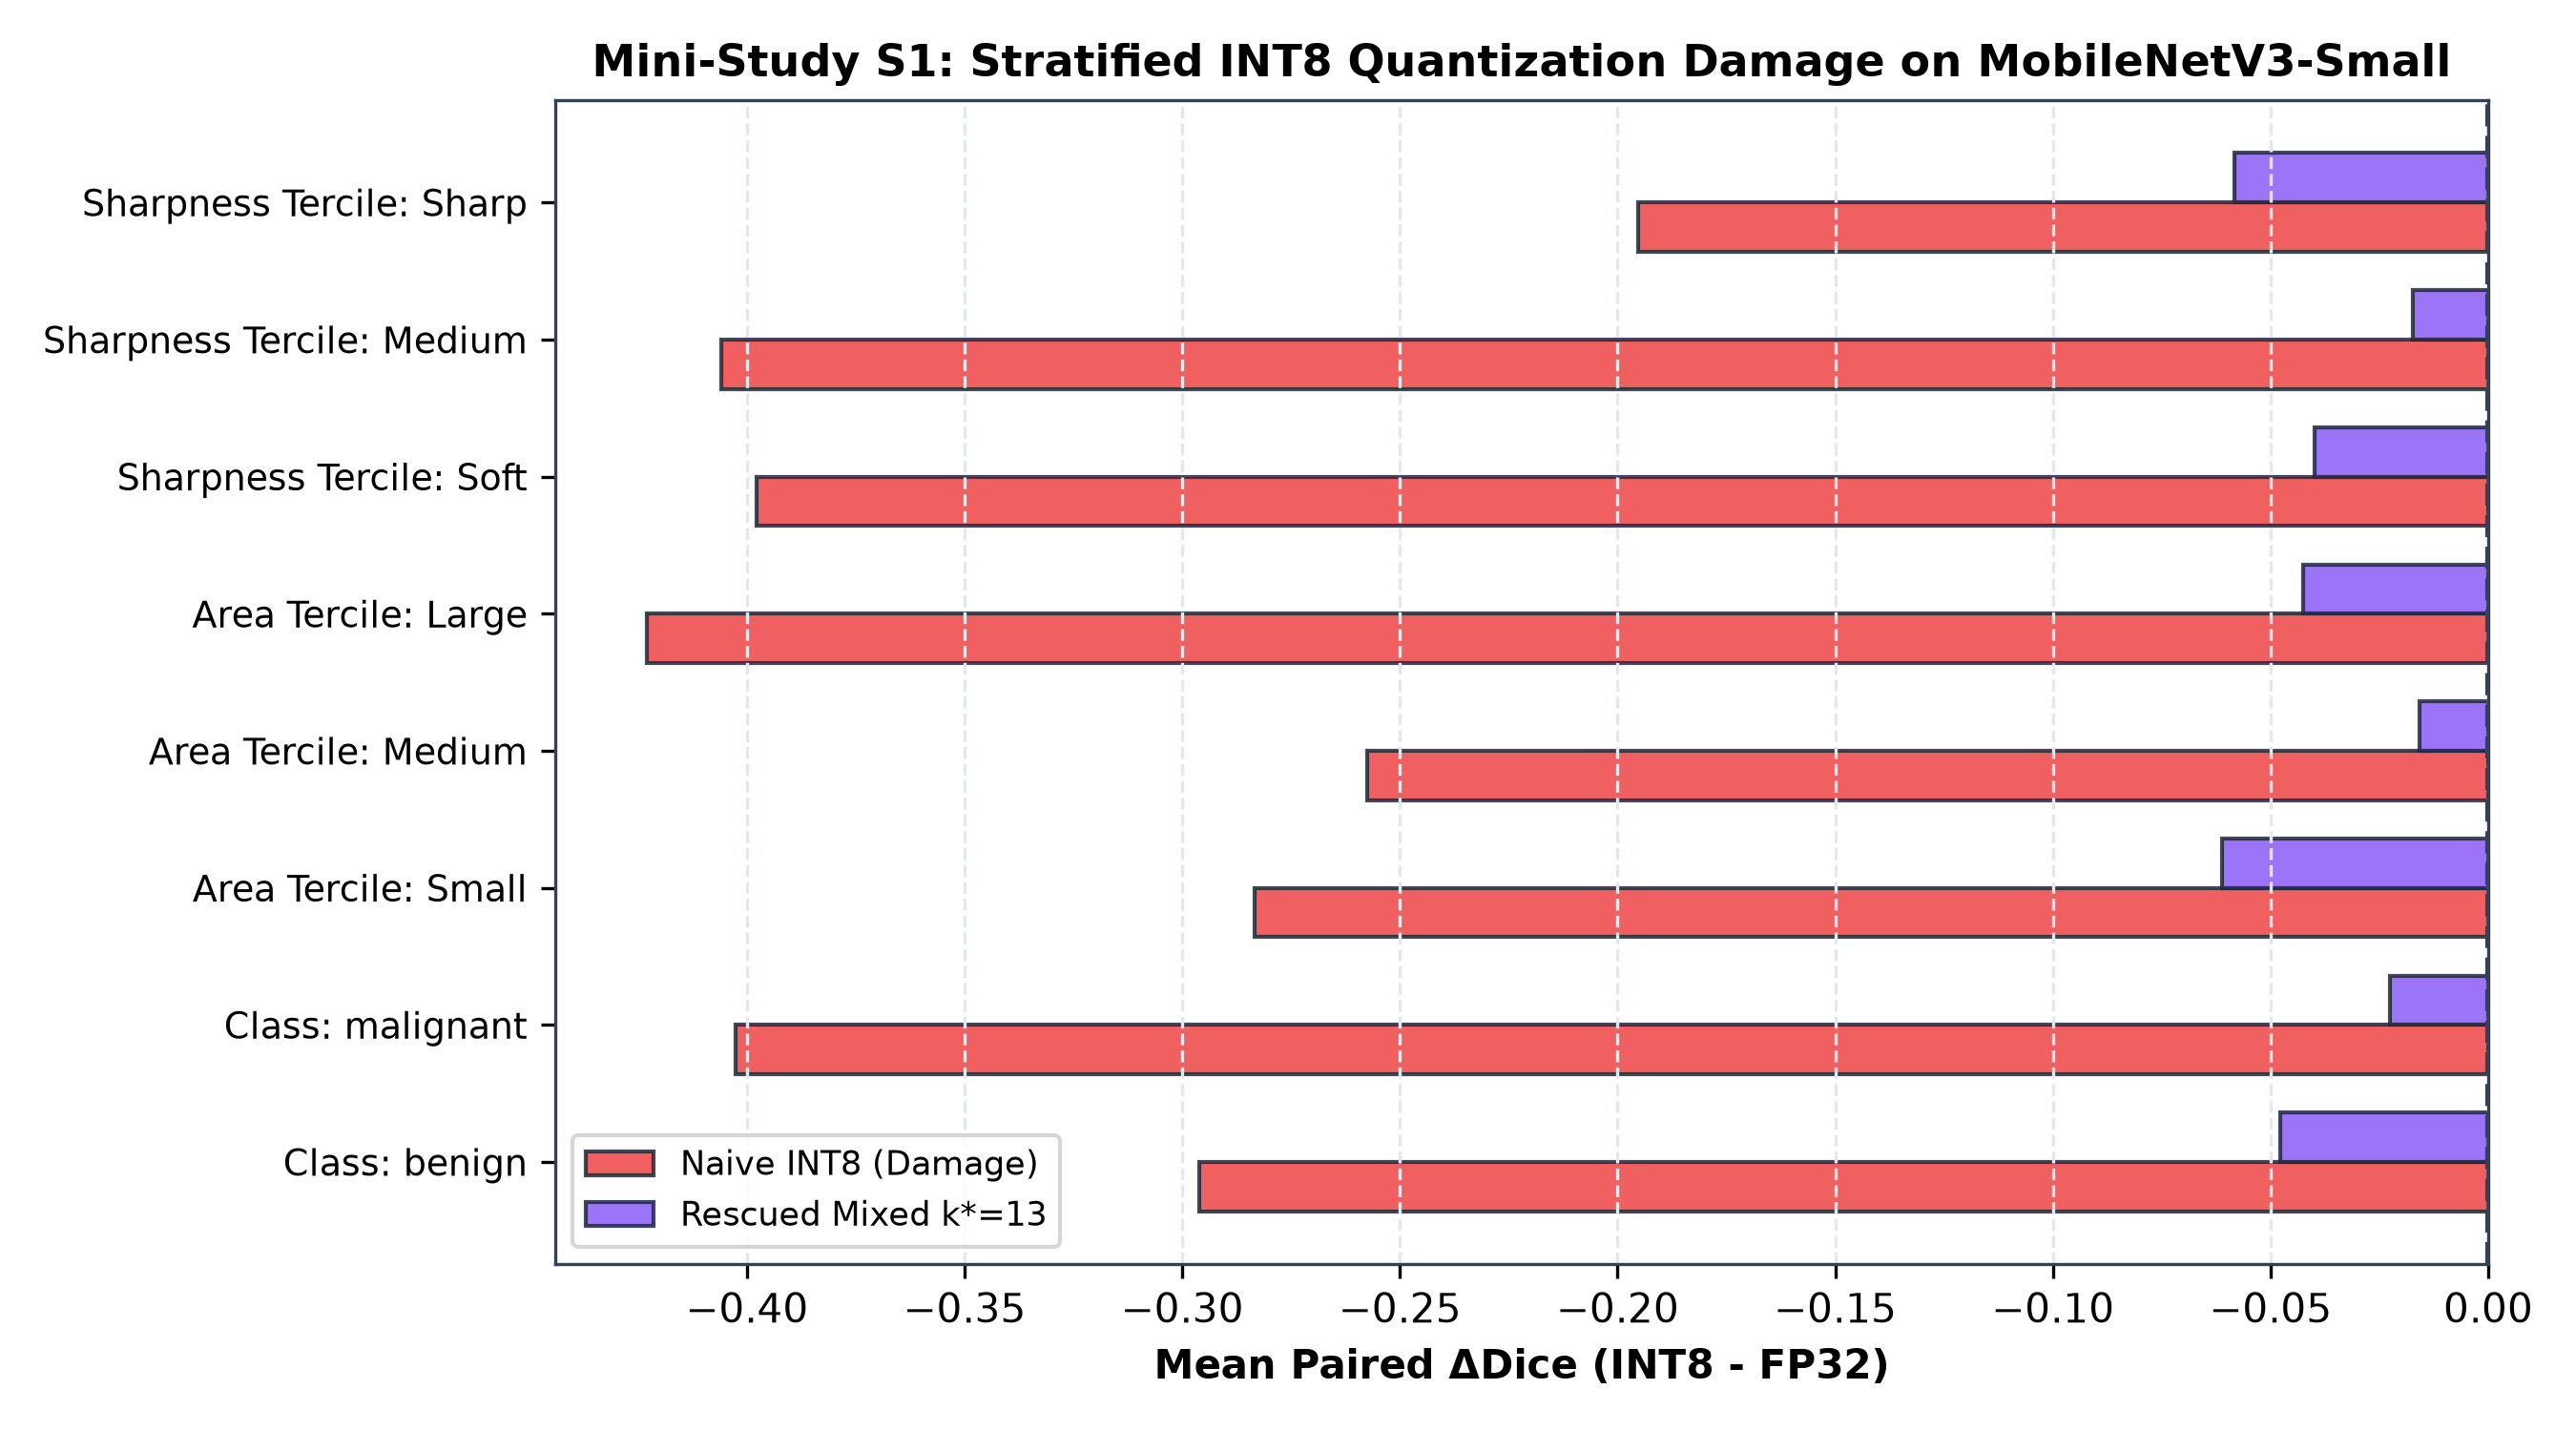
\includegraphics[width=0.95\textwidth,height=0.30\textheight,keepaspectratio]{../figures/study_s1_stratified_damage.png}\\
    \tiny\textcolor{MedSlate}{\textbf{Mini-Study S1:} Soft margins ($\Delta\text{DSC}=-0.40$) and malignant tumors ($-0.40$) suffer up to $2\times$ worse INT8 damage than sharp margins ($-0.20$); Rescued Mixed recovers overall $\Delta\text{DSC}$ to $-0.04$.}
  \end{column}
\end{columns}
\end{frame}

% ==============================================================================
% SLIDE 5: Extension A: Sensitivity Knob & Graph Surgery (Speaker B)
% ==============================================================================
\begin{frame}{Extension A: Mixed-Precision Graph Surgery \& Zero-Recomputation Knob}
\begin{columns}[T]
  \begin{column}{0.52\textwidth}
    \textbf{\footnotesize Diagnosing Layer-Wise Fragility:}
    \vspace{0.1em}
    \begin{itemize}\setlength{\itemsep}{1pt}\scriptsize
      \item Computed empirical \textbf{Signal-to-Quantization-Noise Ratio (SQNR)}:
        $$\textstyle \text{SQNR}_l = 10 \log_{10} \left( \sum_i x_{l,i}^2 / \sum_i (x_{l,i} - \hat{x}_{l,i})^2 \right) \quad [\text{dB}]$$
      \item Structural graph analysis isolated fragile nodes: input/output boundaries and inverted bottleneck depthwise convolutions ($groups > 1$).
    \end{itemize}

    \vspace{-0.2em}
    \begin{exampleblock}{\textbf{Rescued Operating Point ($k^* = 13$)}}
      \scriptsize
      \begin{itemize}\setlength{\itemsep}{1pt}
        \item Preserves just \textbf{13 of 63} convolutions in FP32; quantizes remaining 50 layers to INT8.
        \item \textbf{Test DSC recovers to 0.7263} (Median \textbf{0.8448}) with HD95 = 35.2 px.
        \item Retains \textbf{3.30$\times$ compression} (\textbf{2.50 MB} vs 8.23 MB) at \textbf{42.9 FPS}.
      \end{itemize}
    \end{exampleblock}
  \end{column}

  \begin{column}{0.46\textwidth}
    \centering
    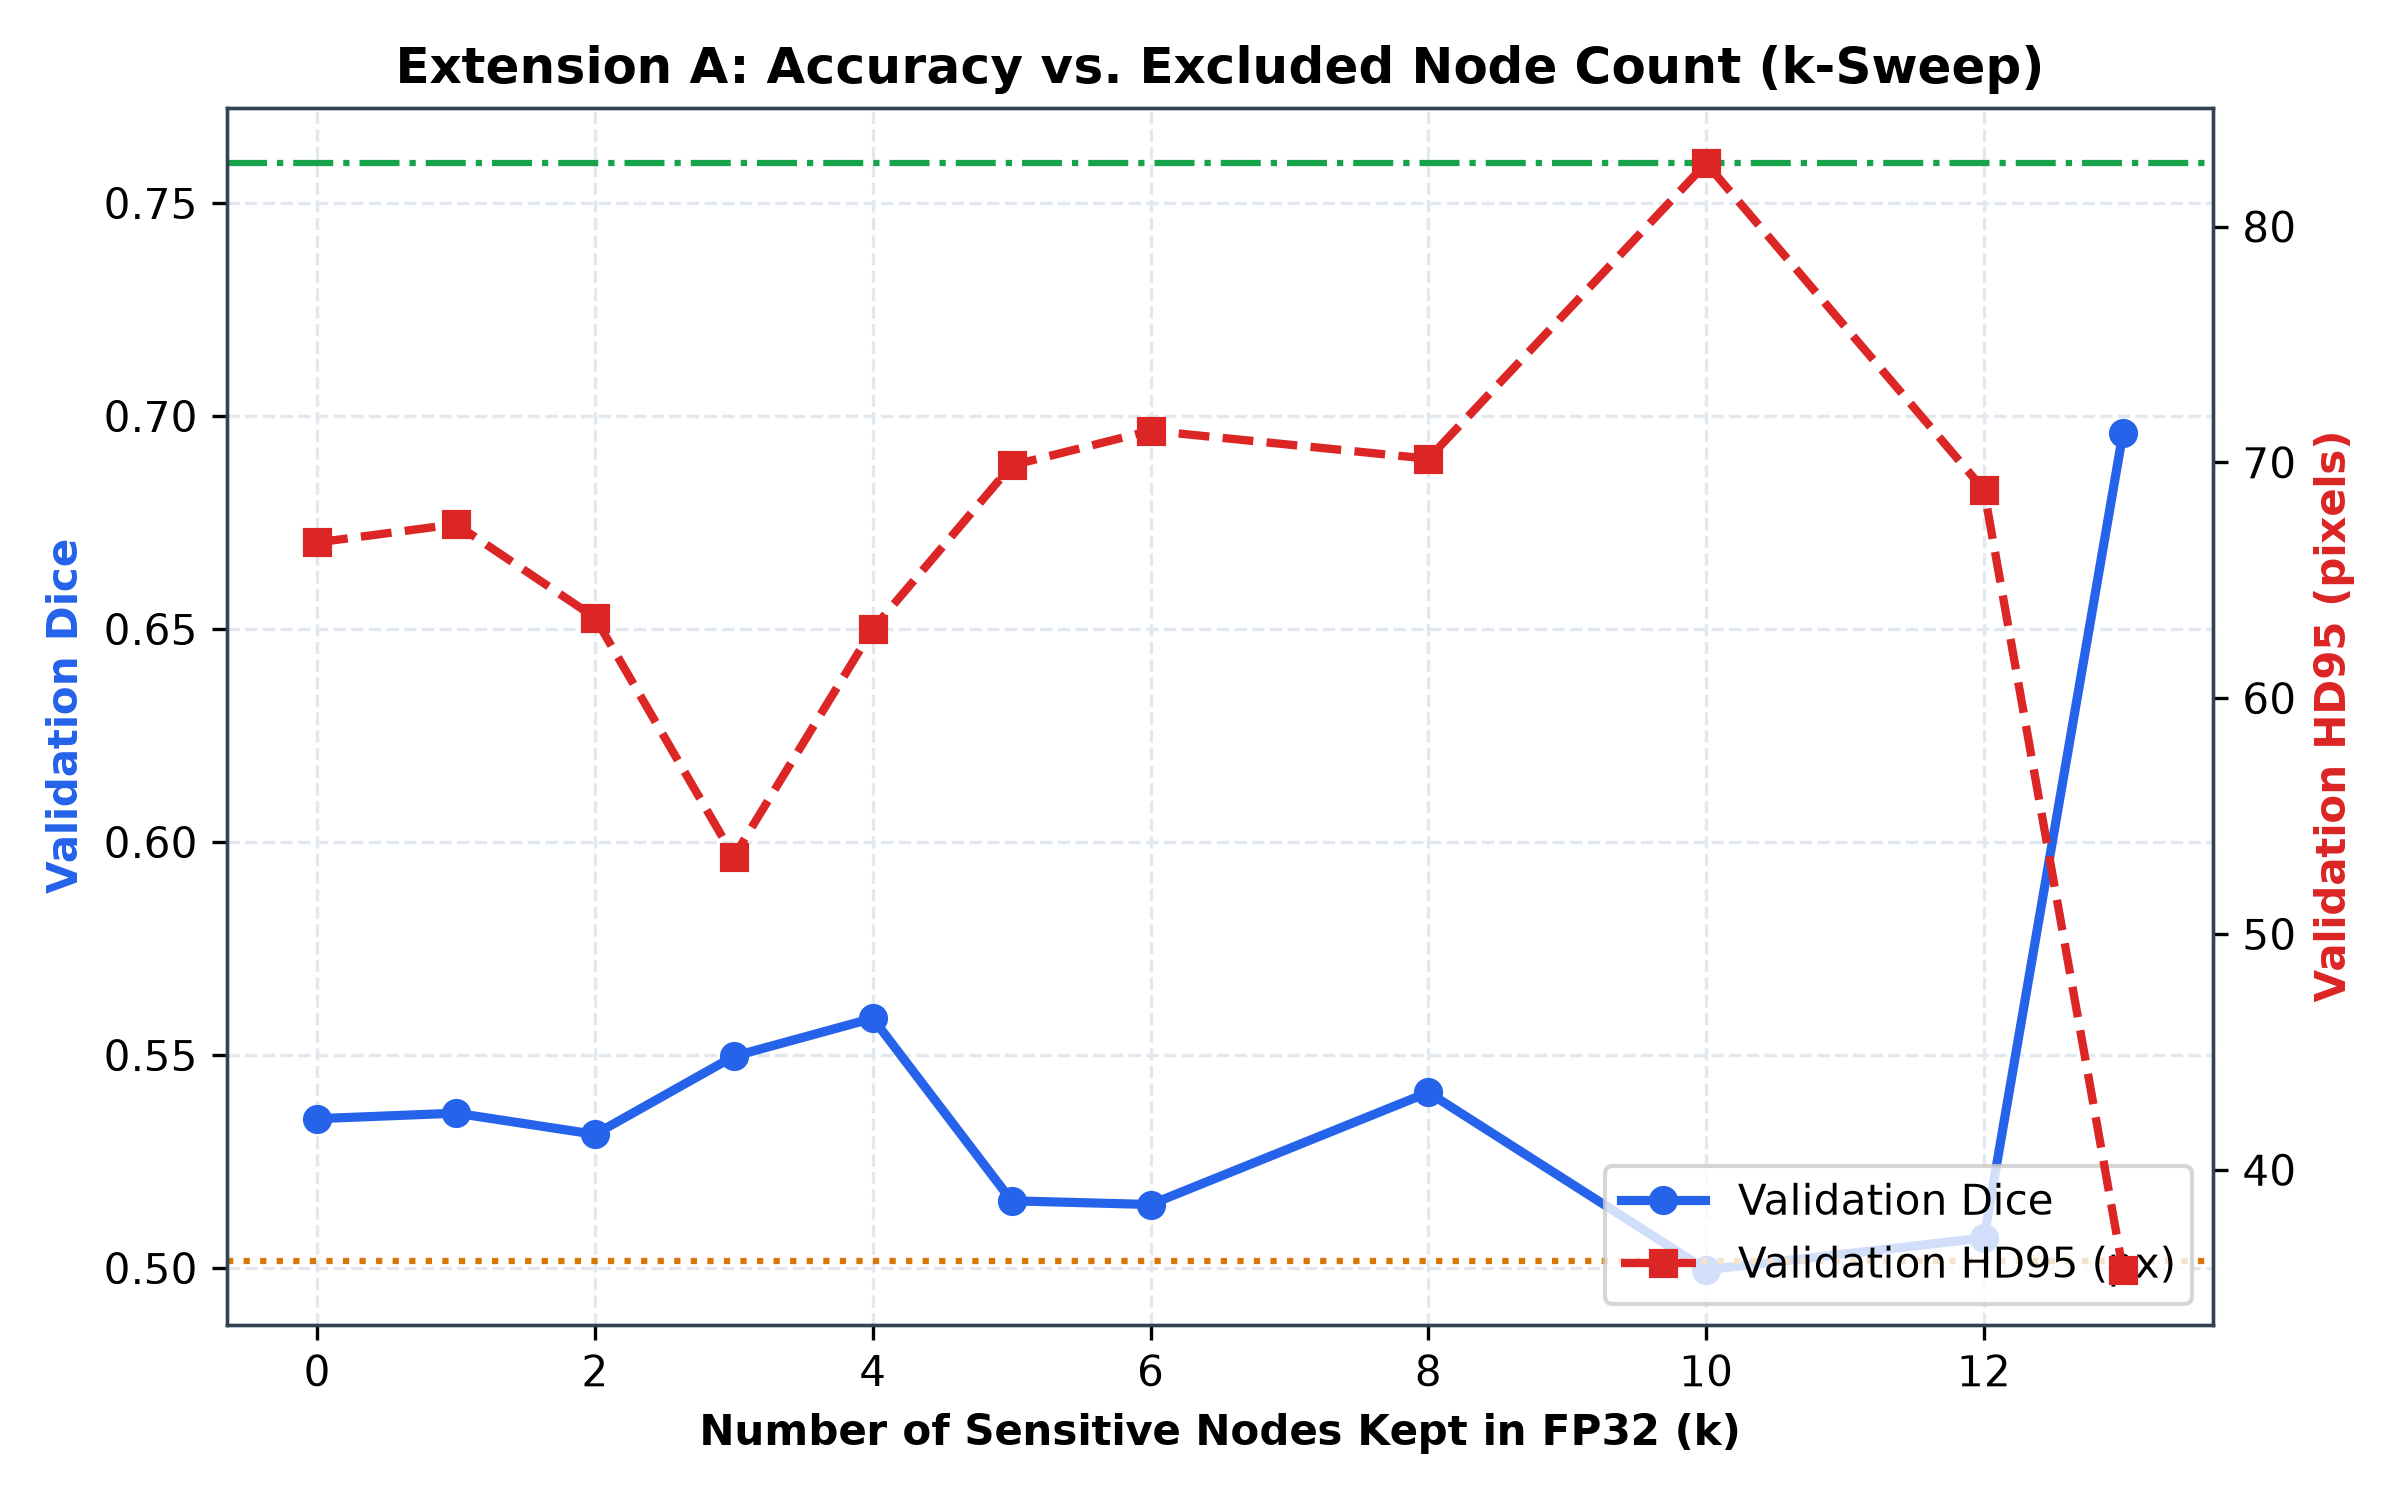
\includegraphics[width=0.95\textwidth,height=0.38\textheight,keepaspectratio]{../figures/extA_k_sweep_curve.png}
    \vspace{-0.2em}
    \begin{block}{\textbf{Zero-Recomputation CLI Knob}}
      \scriptsize Implemented in \texttt{src/quant/knob.py}: Allows sonographers to dynamically dial $k \in [0, 63]$ without retraining weights.
    \end{block}
  \end{column}
\end{columns}
\end{frame}

% ==============================================================================
% SLIDE 6: Knowledge Distillation & Distil-Quantization (Speaker B)
% ==============================================================================
\begin{frame}{Knowledge Distillation: Overcoming Edge Capacity Limits}
\begin{columns}[T]
  \begin{column}{0.52\textwidth}
    \textbf{\footnotesize Teacher-Student Distillation Framework:}
    \vspace{0.1em}
    \begin{itemize}\setlength{\itemsep}{1pt}\scriptsize
      \item \textbf{Teacher:} Pretrained ResNet-34 U-Net (FP32, 24.44M params).
      \item \textbf{Student:} MobileNetV3-Small U-Net (2.15M params).
      \item \textbf{Compound Distillation Objective ($\alpha=0.50, T=2.0$):}
        $$\mathcal{L}_{\text{KD}} = 0.5 \mathcal{L}_{\text{task}} + 0.5 \cdot T^2 \mathcal{L}_{\text{BCE}}\left(\sigma(z_s/T),\; \sigma(z_t/T)\right)$$
        \tiny where $T=2.0$ softens tumor boundary logits to transfer spatial dark knowledge.
    \end{itemize}

    \vspace{-0.2em}
    \begin{exampleblock}{\textbf{Distillation Breakthrough}}
      \scriptsize
      \begin{itemize}\setlength{\itemsep}{1pt}
        \item Distilled MobileNetV3 reaches \textbf{0.8034 DSC} [0.7617, 0.8430] (Median \textbf{0.8916}, HD95 \textbf{26.44 px}).
        \item \textbf{Surpasses the Teacher (0.8012)} with 11.4$\times$ fewer weights!
      \end{itemize}
    \end{exampleblock}
  \end{column}

  \begin{column}{0.46\textwidth}
    \centering
    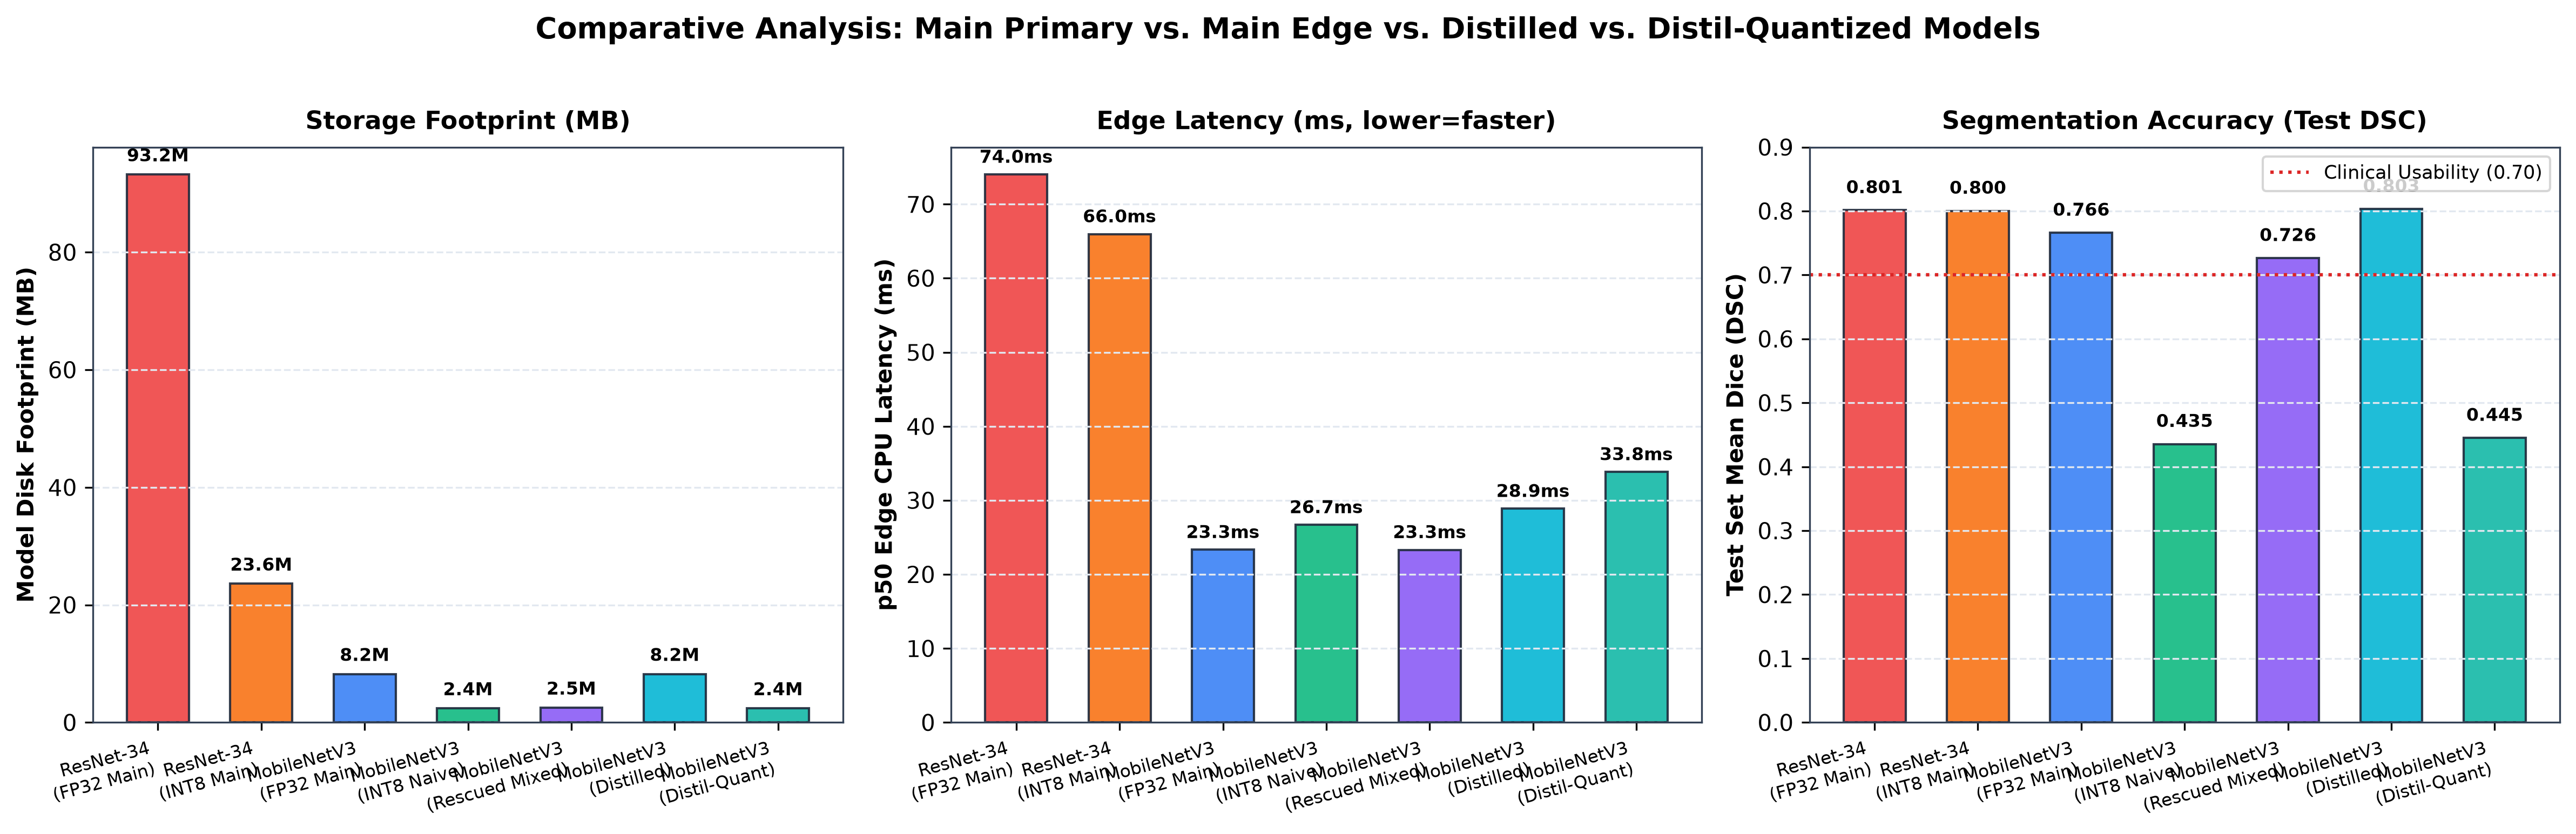
\includegraphics[width=0.98\textwidth,height=0.38\textheight,keepaspectratio]{../figures/distil_quant_main_comparison.png}
    \vspace{-0.3em}
    \begin{alertblock}{\textbf{Distil-Quant Reality Check}}
      \scriptsize Naive INT8 quantization of distilled weights still drops to \textbf{0.4450 DSC}. Distillation alone cannot eliminate depthwise clipping without mixed precision!
    \end{alertblock}
  \end{column}
\end{columns}
\end{frame}

% ==============================================================================
% SLIDE 7: Systems & Operator Profiling Deep-Dive (Speaker B)
% ==============================================================================
\begin{frame}{Systems Profiling: Operator Breakdown \& Latency Bottlenecks}
\begin{columns}[T]
  \begin{column}{0.48\textwidth}
    \centering
    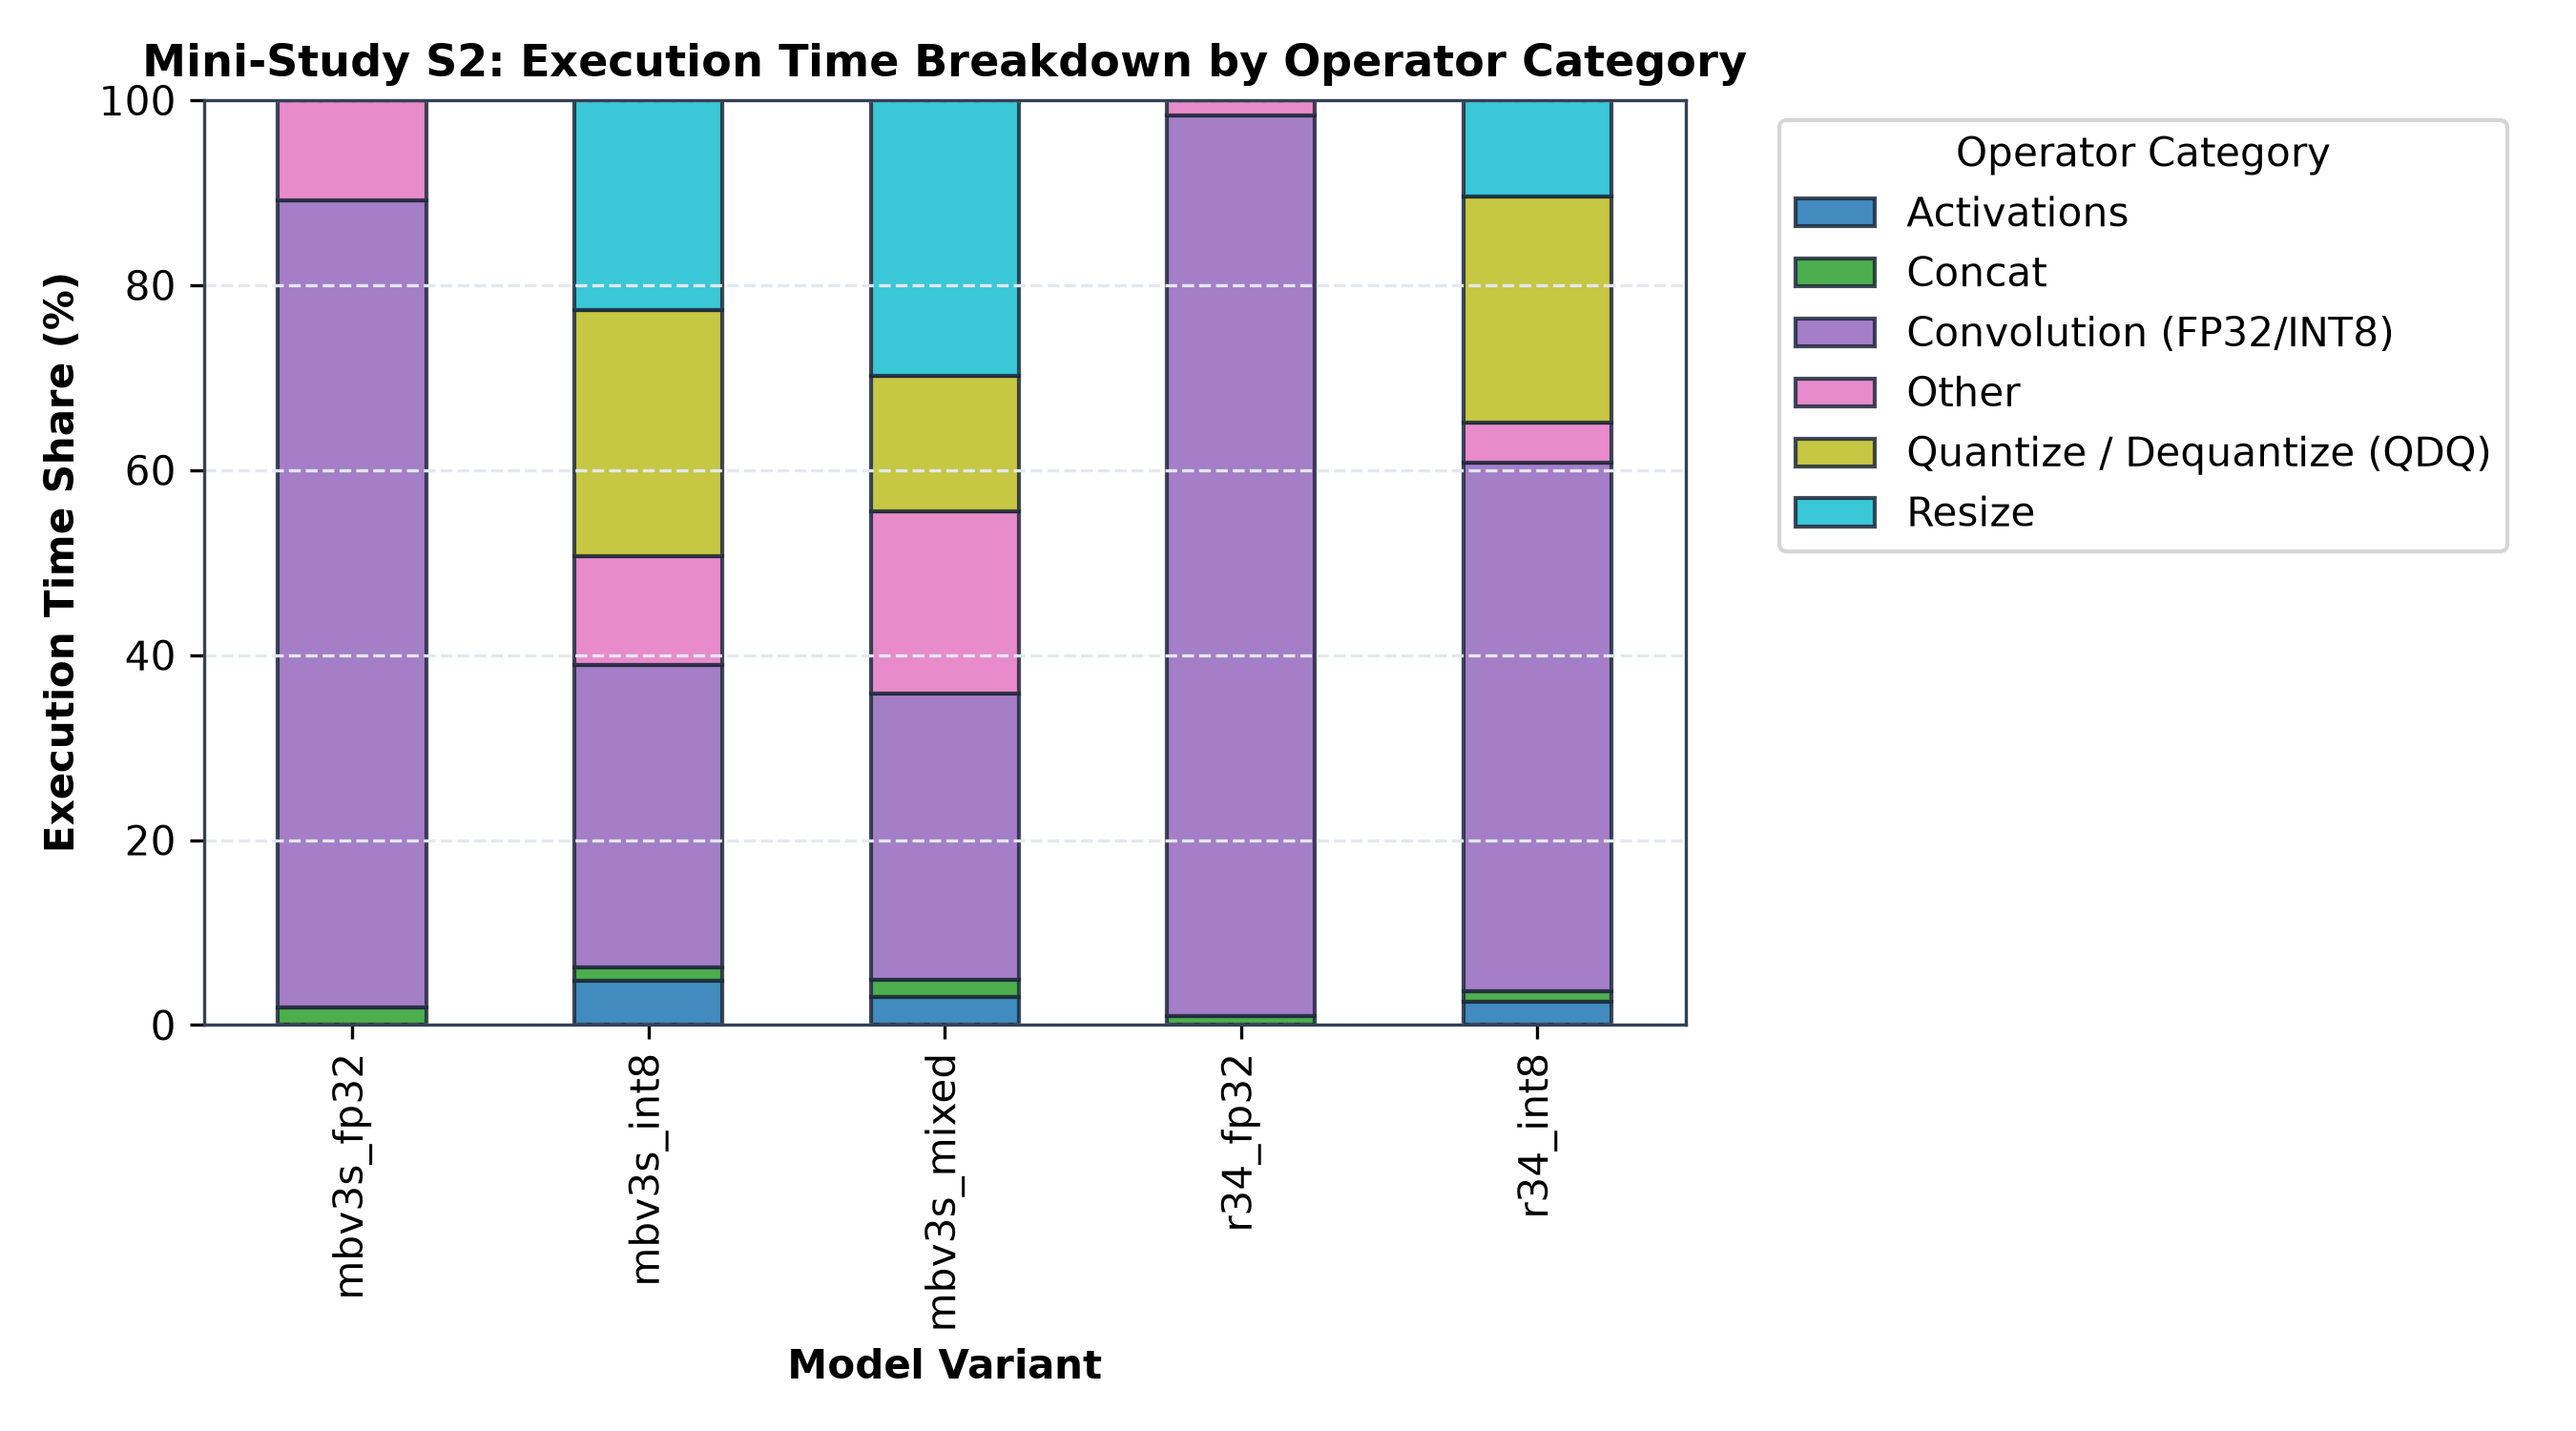
\includegraphics[width=0.98\textwidth,height=0.55\textheight,keepaspectratio]{../figures/study_s2_operator_breakdown.png}\\
    \tiny\textcolor{MedSlate}{\textbf{Mini-Study S2:} Execution time distribution by ONNX operator category.}
  \end{column}

  \begin{column}{0.50\textwidth}
    \textbf{\footnotesize Systems Telemetry Insights (Mini-Study S2):}
    \vspace{0.1em}
    \begin{itemize}\setlength{\itemsep}{1pt}\scriptsize
      \item In standard INT8 networks, GEMM/Convolutions are expected to dominate runtime.
      \item \textbf{The QDQ Bottleneck:} In Naive INT8 MobileNetV3, \textbf{QuantizeLinear and DequantizeLinear nodes consumed 26.6\% of total runtime}!
      \item Memory bandwidth and frequent casting between INT8 and FP32 negate integer MAC gains on lightweight architectures.
    \end{itemize}

    \vspace{0.2em}
    \begin{exampleblock}{\textbf{Why Rescued Mixed is Faster than Naive INT8}}
      \scriptsize
      \begin{itemize}\setlength{\itemsep}{1pt}
        \item By pruning QDQ nodes around the 13 most fragile layers, \textbf{QDQ overhead drops to 14.6\%}.
        \item Eliminating unnecessary boundary conversions allows Rescued Mixed (\textbf{23.31 ms}) to run faster than Naive INT8 (\textbf{26.68 ms})!
      \end{itemize}
    \end{exampleblock}
  \end{column}
\end{columns}
\end{frame}

% ==============================================================================
% SLIDE 8: Master Quantitative Results & Pareto Frontier (Speaker C)
% ==============================================================================
\begin{frame}{Master Quantitative Results: Held-Out BUSI Test Evaluation}
\vspace{-0.5em}
\begin{table}[h]
\centering
\fontsize{6pt}{7pt}\selectfont
\setlength{\tabcolsep}{3pt}
\begin{tabular}{lcccccc}
\toprule
\textbf{Model \& Precision Variant} & \textbf{Params} & \textbf{Size (MB)} & \textbf{Latency} & \textbf{FPS} & \textbf{Mean DSC [95\% CI]} & \textbf{HD95 (px)} \\
\midrule
ResNet-34 FP32 (Teacher) & 24.44M & 93.22 & 74.0 ms & 13.5 & 0.8012 [0.7535, 0.8457] & 27.71 \\
\textbf{ResNet-34 Static INT8 (Ours)} & 24.44M & \textbf{23.59} & 66.0 ms & 15.2 & \textbf{0.8003} [0.7515, 0.8462] & 28.56 \\
MobileNetV3 FP32 (Edge Baseline) & 2.15M & 8.23 & 23.3 ms & 42.9 & 0.7659 [0.7123, 0.8163] & 35.13 \\
MobileNetV3 Static INT8 (Naive) & 2.15M & 2.39 & 26.7 ms & 37.5 & 0.4355 [0.3612, 0.5002] & 86.97 \\
\textbf{MobileNetV3 Rescued Mixed ($k^*=13$)} & 2.15M & \textbf{2.50} & \textbf{23.3 ms} & \textbf{42.9} & \textbf{0.7263} [0.6690, 0.7784] & \textbf{35.20} \\
\textbf{MobileNetV3 Distilled FP32 (Ours)} & \textbf{2.15M} & \textbf{8.23} & \textbf{28.9 ms} & \textbf{34.9} & \textbf{0.8034} [0.7617, 0.8430] & \textbf{26.44} \\
MobileNetV3 Distilled INT8 (Naive) & 2.15M & 2.39 & 33.8 ms & 29.7 & 0.4450 [0.3810, 0.5080] & 82.64 \\
\bottomrule
\end{tabular}
\end{table}

\vspace{-0.4em}
\begin{columns}[T]
  \begin{column}{0.48\textwidth}
    \centering
    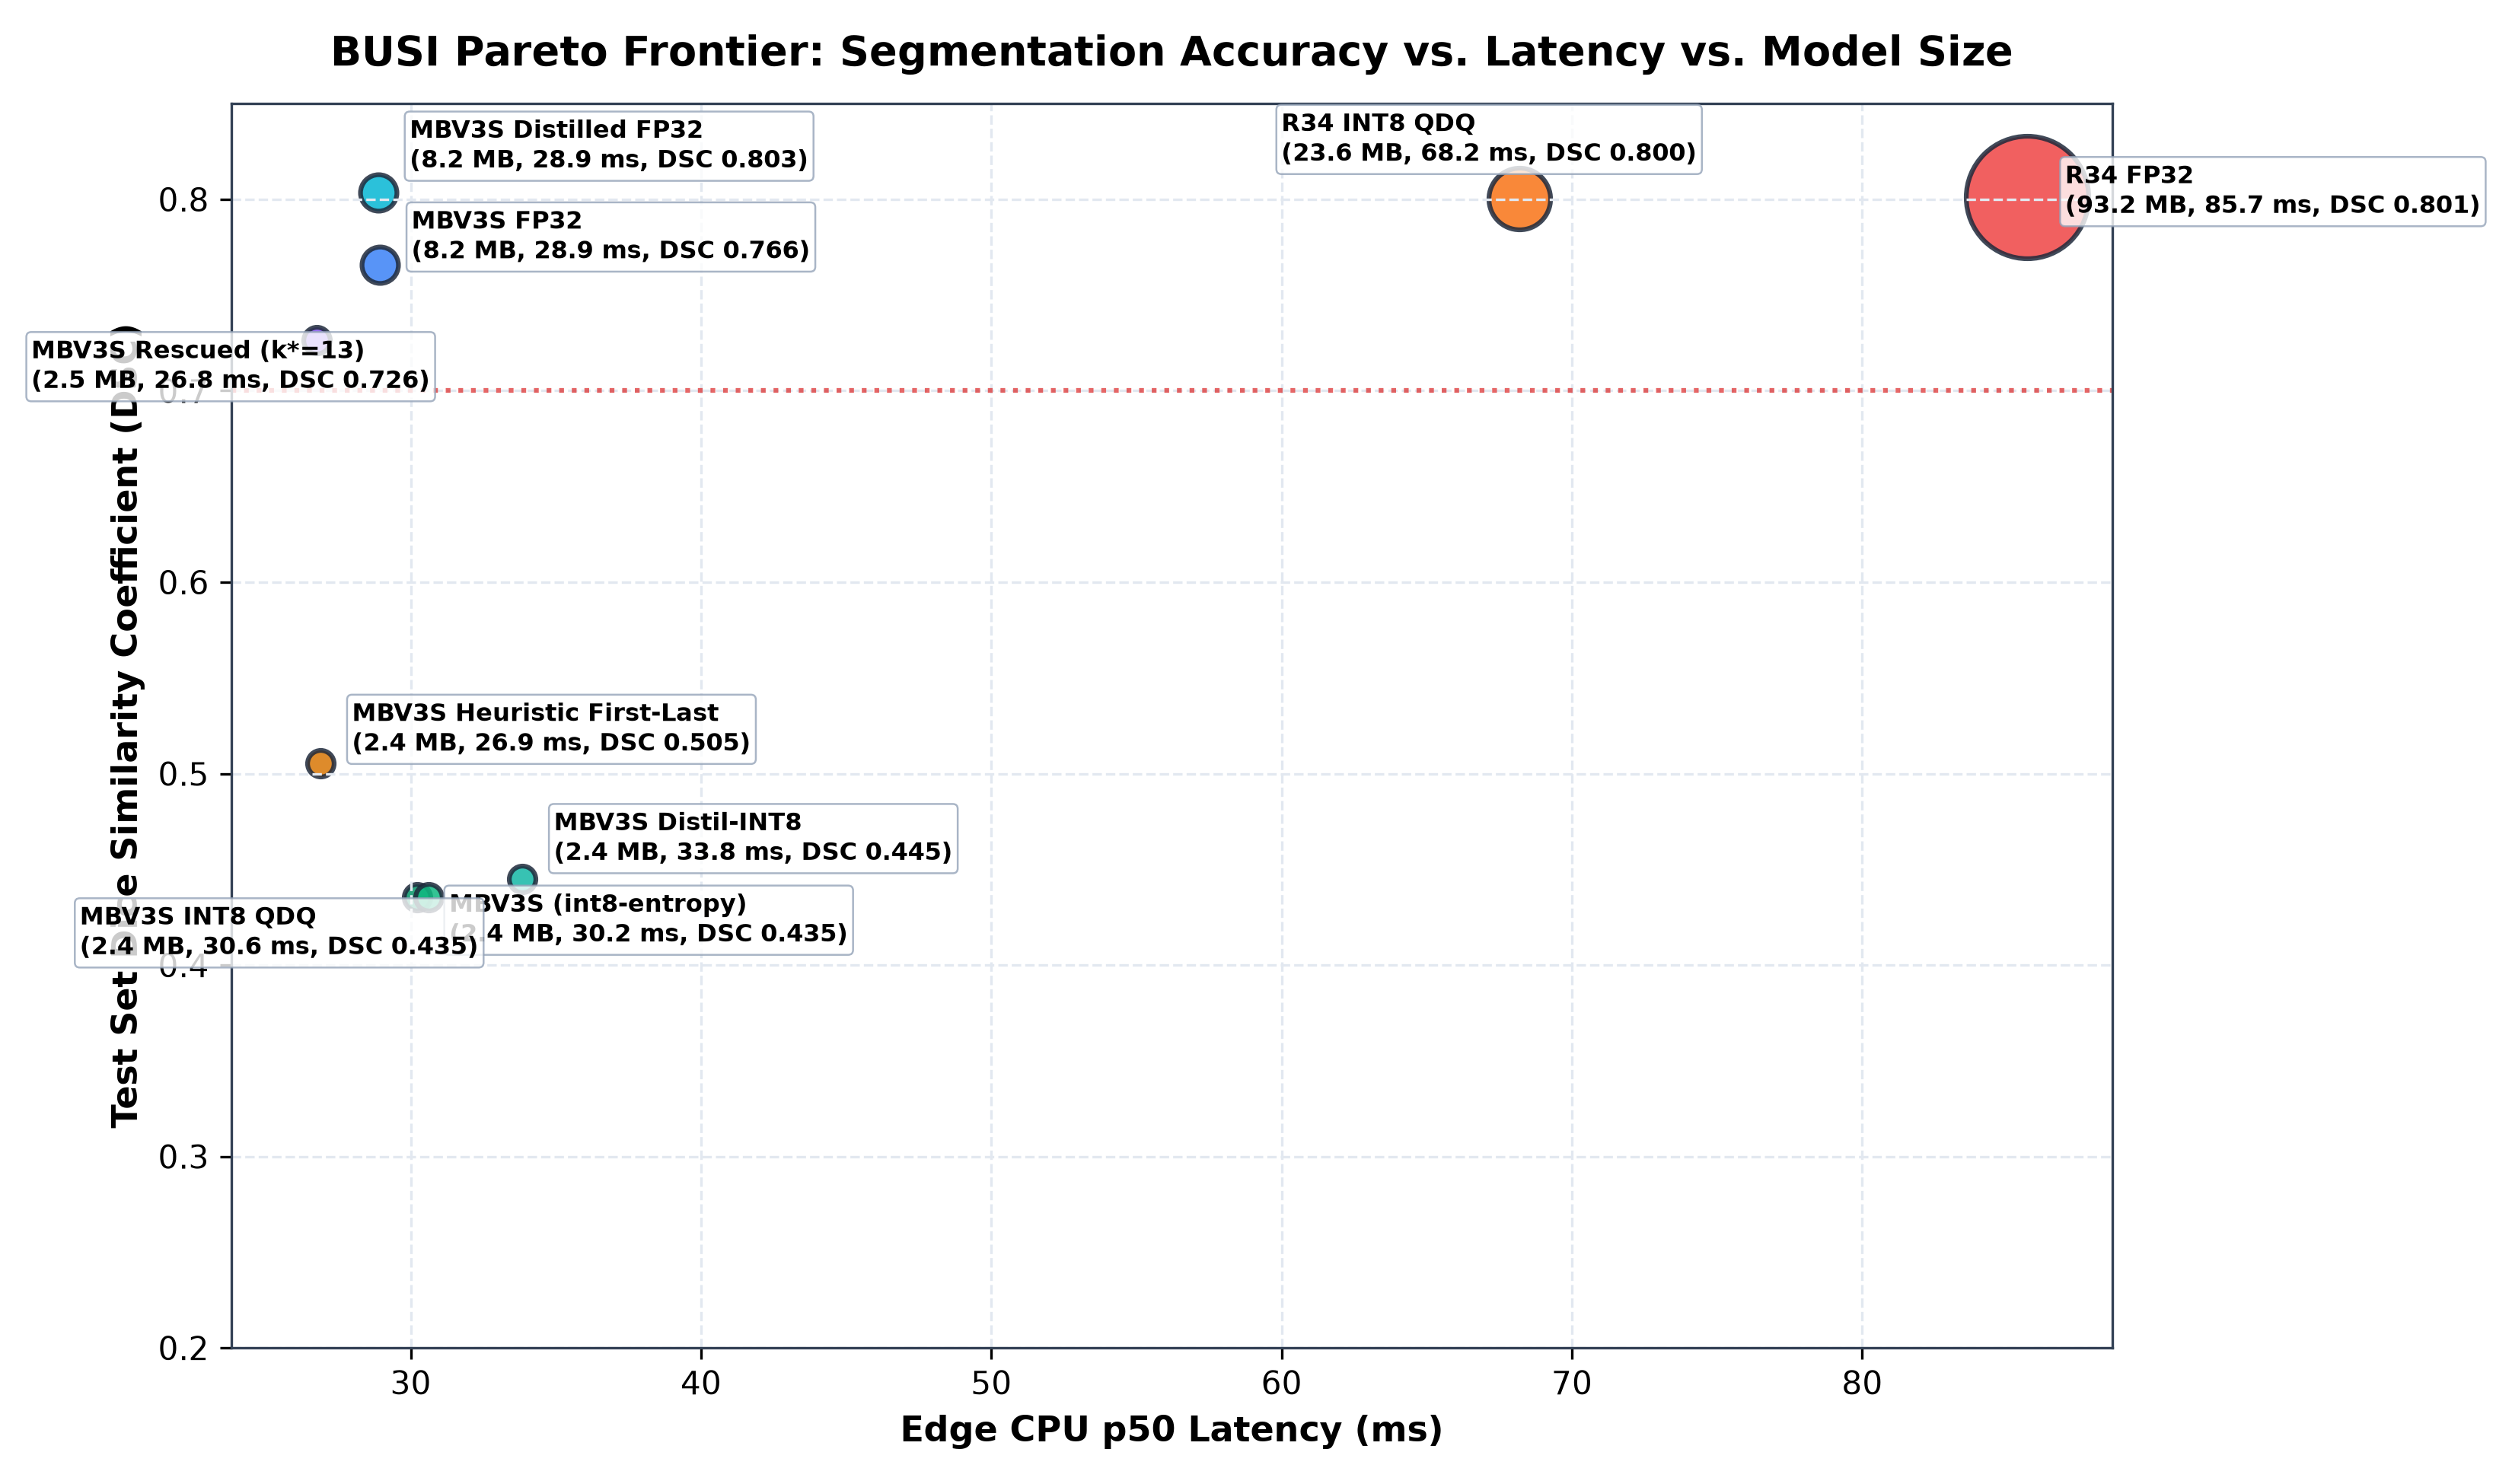
\includegraphics[width=0.98\textwidth,height=0.42\textheight,keepaspectratio]{../figures/pareto_dice_vs_latency.png}
  \end{column}

  \begin{column}{0.50\textwidth}
    \vspace{0.1em}
    \textbf{\scriptsize Three Optimal Operating Modes on the Frontier:}
    \begin{enumerate}\setlength{\itemsep}{1pt}\scriptsize
      \item \textbf{Lossless Diagnostic Quality:} ResNet-34 INT8 (0.8003 DSC, 23.6 MB, 15.2 FPS).
      \item \textbf{Peak Lightweight Accuracy:} MobileNetV3 Distilled (0.8034 DSC, 8.23 MB, 34.9 FPS).
      \item \textbf{Ultra-Compact Edge Streaming:} MobileNetV3 Rescued Mixed (0.7263 DSC, 2.50 MB, 42.9 FPS).
    \end{enumerate}
  \end{column}
\end{columns}
\end{frame}

% ==============================================================================
% SLIDE 9: Literature Benchmark & Cross-Center Generalization (Speaker C)
% ==============================================================================
\begin{frame}{Literature Benchmark \& Cross-Center Generalization}
\begin{columns}[T]
  \begin{column}{0.50\textwidth}
    \textbf{\scriptsize Comparison with Published State-of-the-Art:}
    \vspace{0.1em}
    \begin{table}[h]
    \centering
    \fontsize{5.5pt}{6.5pt}\selectfont
    \setlength{\tabcolsep}{2.5pt}
    \begin{tabular}{lcccc}
    \toprule
    \textbf{Model / Architecture} & \textbf{Params} & \textbf{Test DSC} & \textbf{Test IoU} & \textbf{Throughput} \\
    \midrule
    Shifaa U-Net (HuggingFace) & 1.94M & 0.4973 & 0.3673 & 17.3 FPS \\
    Attention U-Net (Yap et al.) & 24.55M & 0.7412 & 0.6385 & 7.1 FPS \\
    U-Net++ (Al-Dhabyani et al.) & 26.08M & 0.7588 & 0.6542 & 4.0 FPS \\
    \midrule
    \textbf{Our ResNet-34 INT8} & 24.44M & \textbf{0.8003} & \textbf{0.7187} & \textbf{15.2 FPS} \\
    \textbf{Our MobileNetV3 FP32} & \textbf{2.15M} & \textbf{0.7659} & \textbf{0.6770} & \textbf{42.9 FPS} \\
    \textbf{Our MobileNetV3 Distilled} & \textbf{2.15M} & \textbf{0.8034} & \textbf{0.7042} & \textbf{34.9 FPS} \\
    \textbf{Our MobileNetV3 Rescued} & \textbf{2.15M} & \textbf{0.7263} & \textbf{0.6314} & \textbf{42.9 FPS} \\
    \bottomrule
    \end{tabular}
    \end{table}

    \vspace{-0.3em}
    \begin{block}{\textbf{Cross-Center Zero-Shot Generalization}}
      \scriptsize Tested on \textbf{UDIAT Dataset B (Sabadell, Spain; 163 scans)}:
      \begin{itemize}\setlength{\itemsep}{0pt}\scriptsize
        \item \textbf{ResNet-34 INT8:} Achieves \textbf{0.7928 DSC} (exceeds FP32 0.7902; fine-tuned hits \textbf{0.8283}).
        \item \textbf{MobileNetV3 Rescued:} Sustains \textbf{0.7002 DSC} (Median \textbf{0.8562}) vs Naive INT8 collapse (0.1519).
      \end{itemize}
    \end{block}
  \end{column}

  \begin{column}{0.48\textwidth}
    \centering
    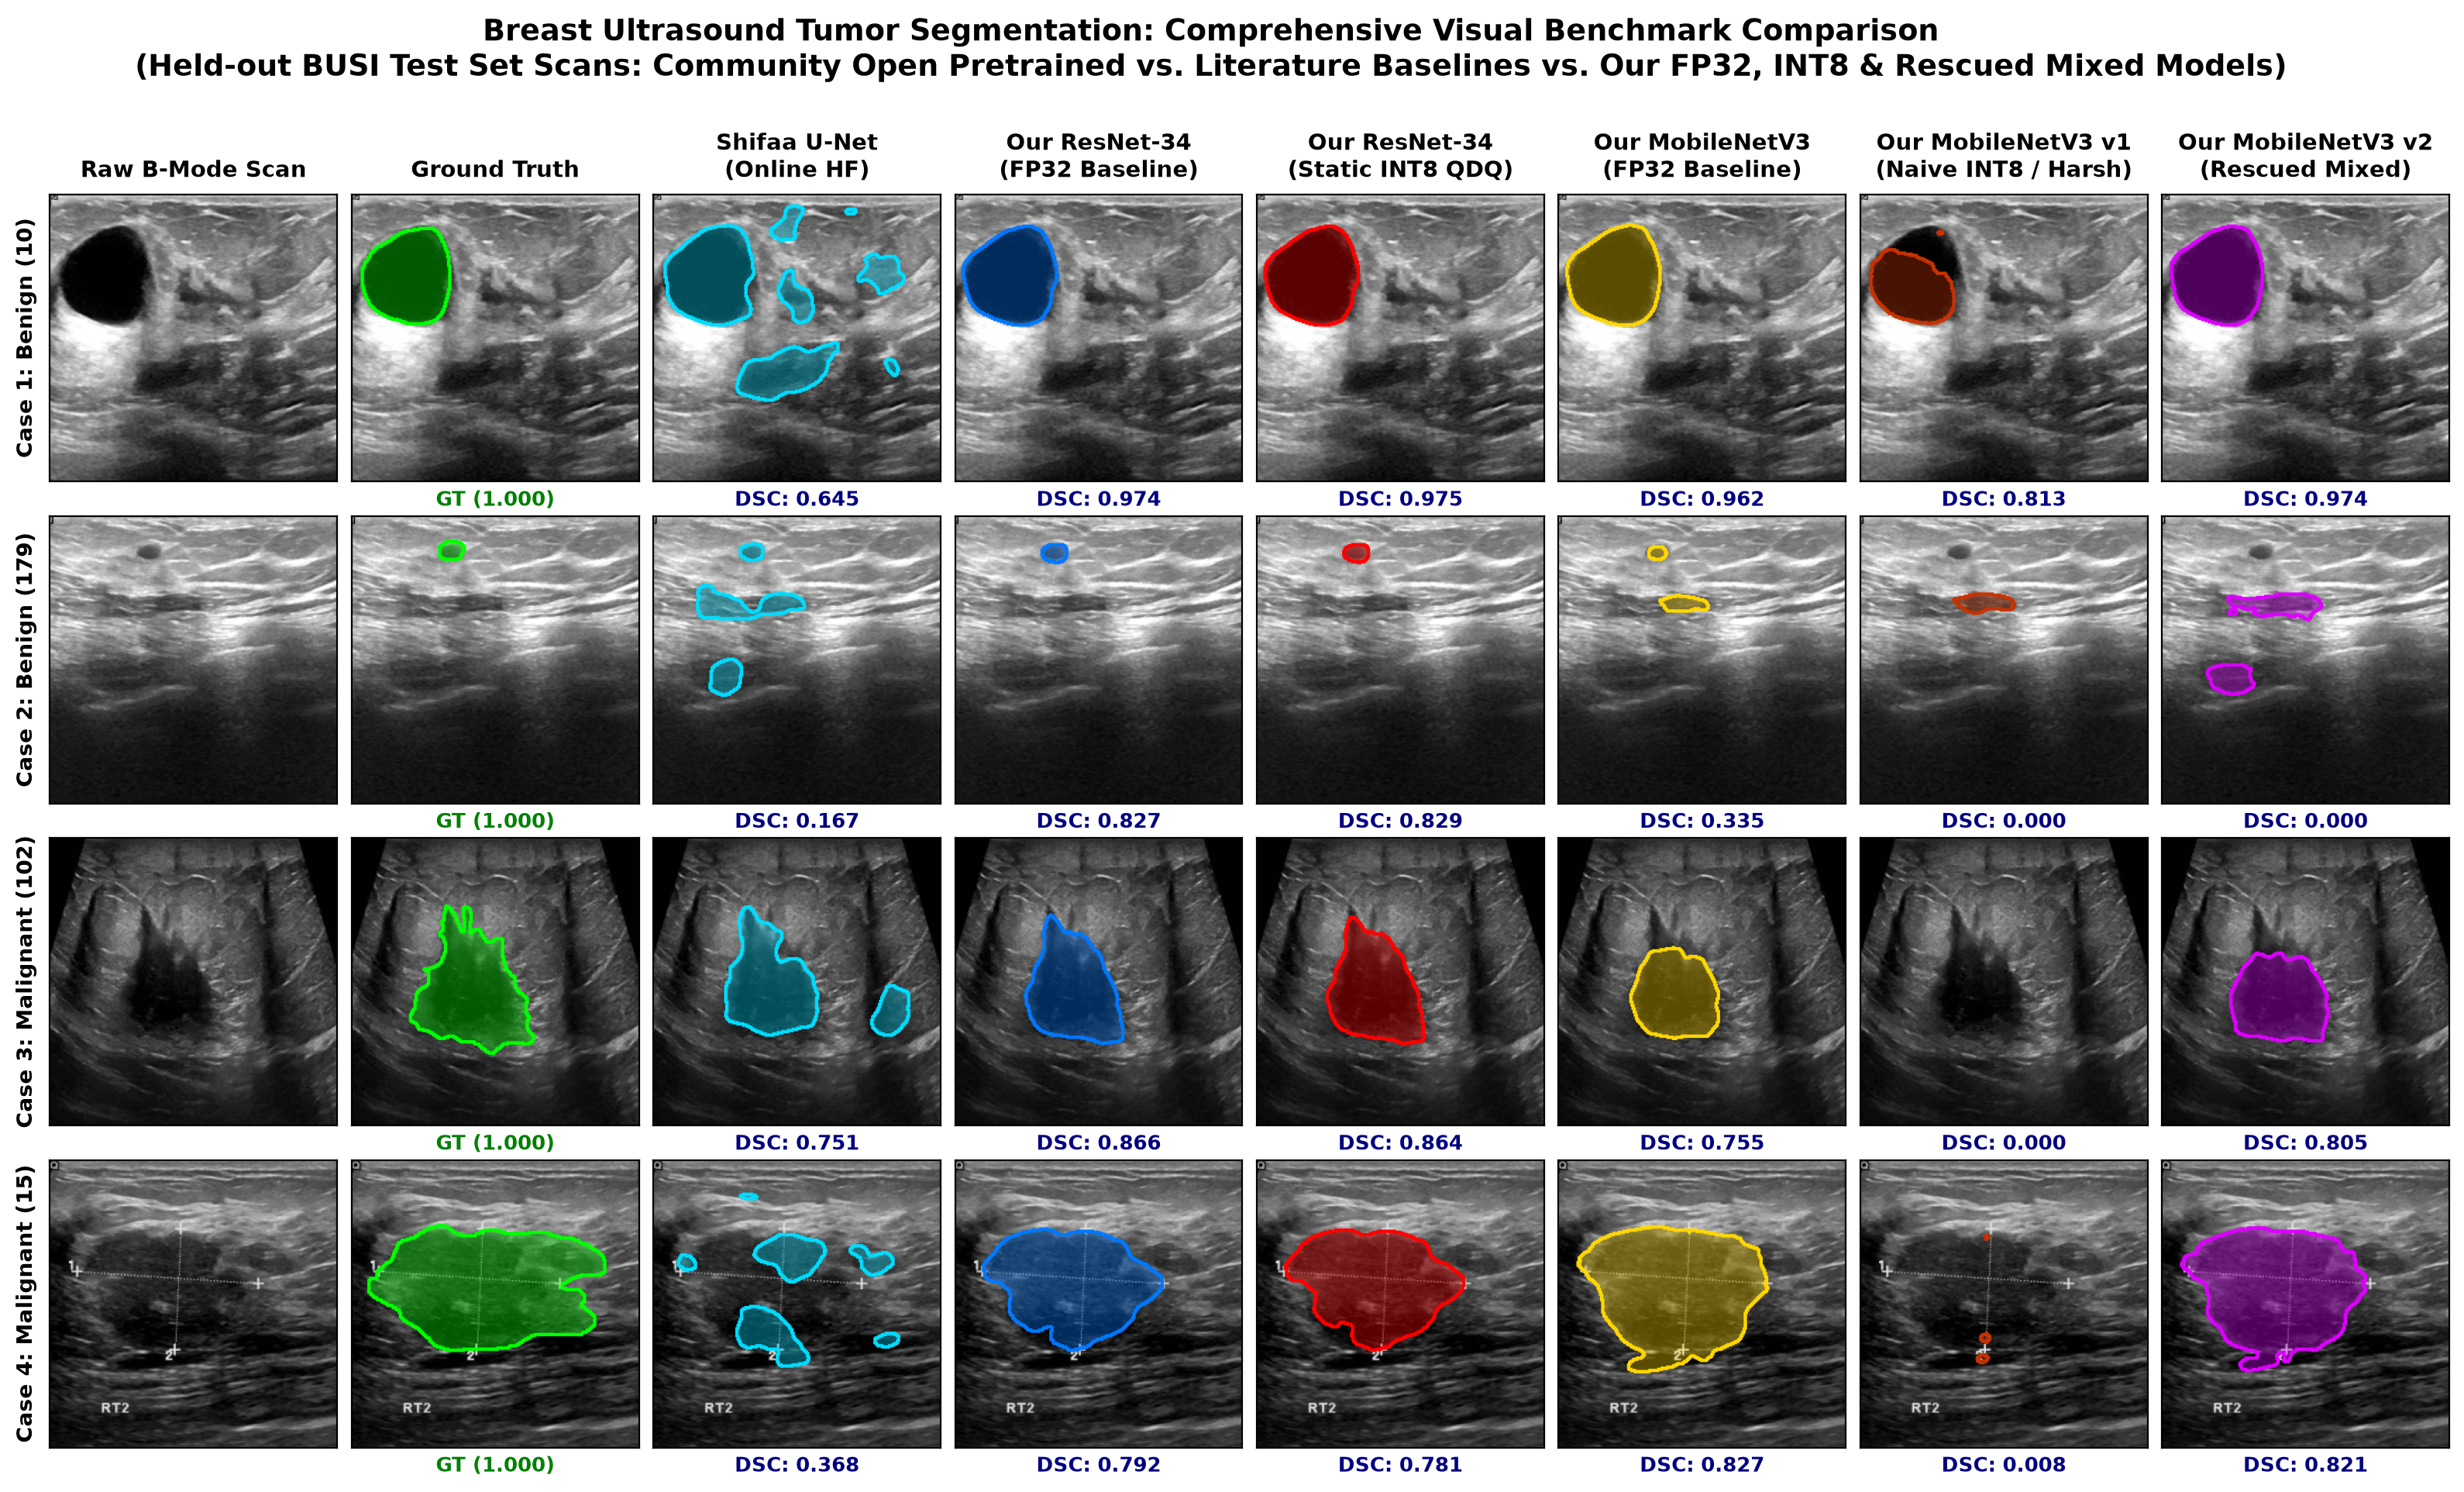
\includegraphics[width=0.98\textwidth,height=0.60\textheight,keepaspectratio]{../figures/benchmark_overlay_comparison.png}\\
    \tiny\textcolor{MedSlate}{\textbf{Qualitative Overlays:} Shifaa U-Net vs Ours across 4 test cases.}
  \end{column}
\end{columns}
\end{frame}

% ==============================================================================
% SLIDE 10: Extension B: Cine Streaming & Temporal Smoothing (Speaker C)
% ==============================================================================
\begin{frame}{Extension B: Real-Time Cine-Loop Streaming \& Temporal Filtering}
\begin{columns}[T]
  \begin{column}{0.50\textwidth}
    \textbf{\footnotesize Multi-Threaded Producer-Consumer Architecture:}
    \vspace{0.1em}
    \begin{itemize}\setlength{\itemsep}{1pt}\scriptsize
      \item Sonographers sweep probes continuously at 30 Hz.
      \item \textbf{Lock-Free Ring Buffer ($C = 4$):} Implements drop-oldest semantics; guarantees frame staleness $\le 33.3$ ms.
      \item \textbf{Benchmark Results at 30 Hz Stream Rate:}
        \begin{itemize}\setlength{\itemsep}{0pt}\scriptsize
          \item MobileNetV3 FP32 \& Rescued: \textbf{0.02\%--0.06\% drops} ($\sim$29 ms e2e).
          \item ResNet-34 INT8 \& FP32: \textbf{56.3\% to 61.9\% frame drops} (cannot sustain live feeds).
        \end{itemize}
    \end{itemize}

    \vspace{-0.2em}
    \begin{block}{\textbf{Temporal EMA Logit Smoothing ($\alpha = 0.60$)}}
      \scriptsize
      $$Z_t^{\text{EMA}} = \alpha Z_t + (1-\alpha) Z_{t-1}^{\text{EMA}}$$
      Evaluated on genuine clinical videos (UFUV MICCAI cohort):
      \begin{itemize}\setlength{\itemsep}{0pt}\scriptsize
        \item Eliminates high-frequency boundary flicker.
        \item Boosts Temporal Consistency Index (TCI) by \textbf{+18.5\% to +65.2\%} (mean \textbf{+37.7\%}).
      \end{itemize}
    \end{block}
  \end{column}

  \begin{column}{0.48\textwidth}
    \centering
    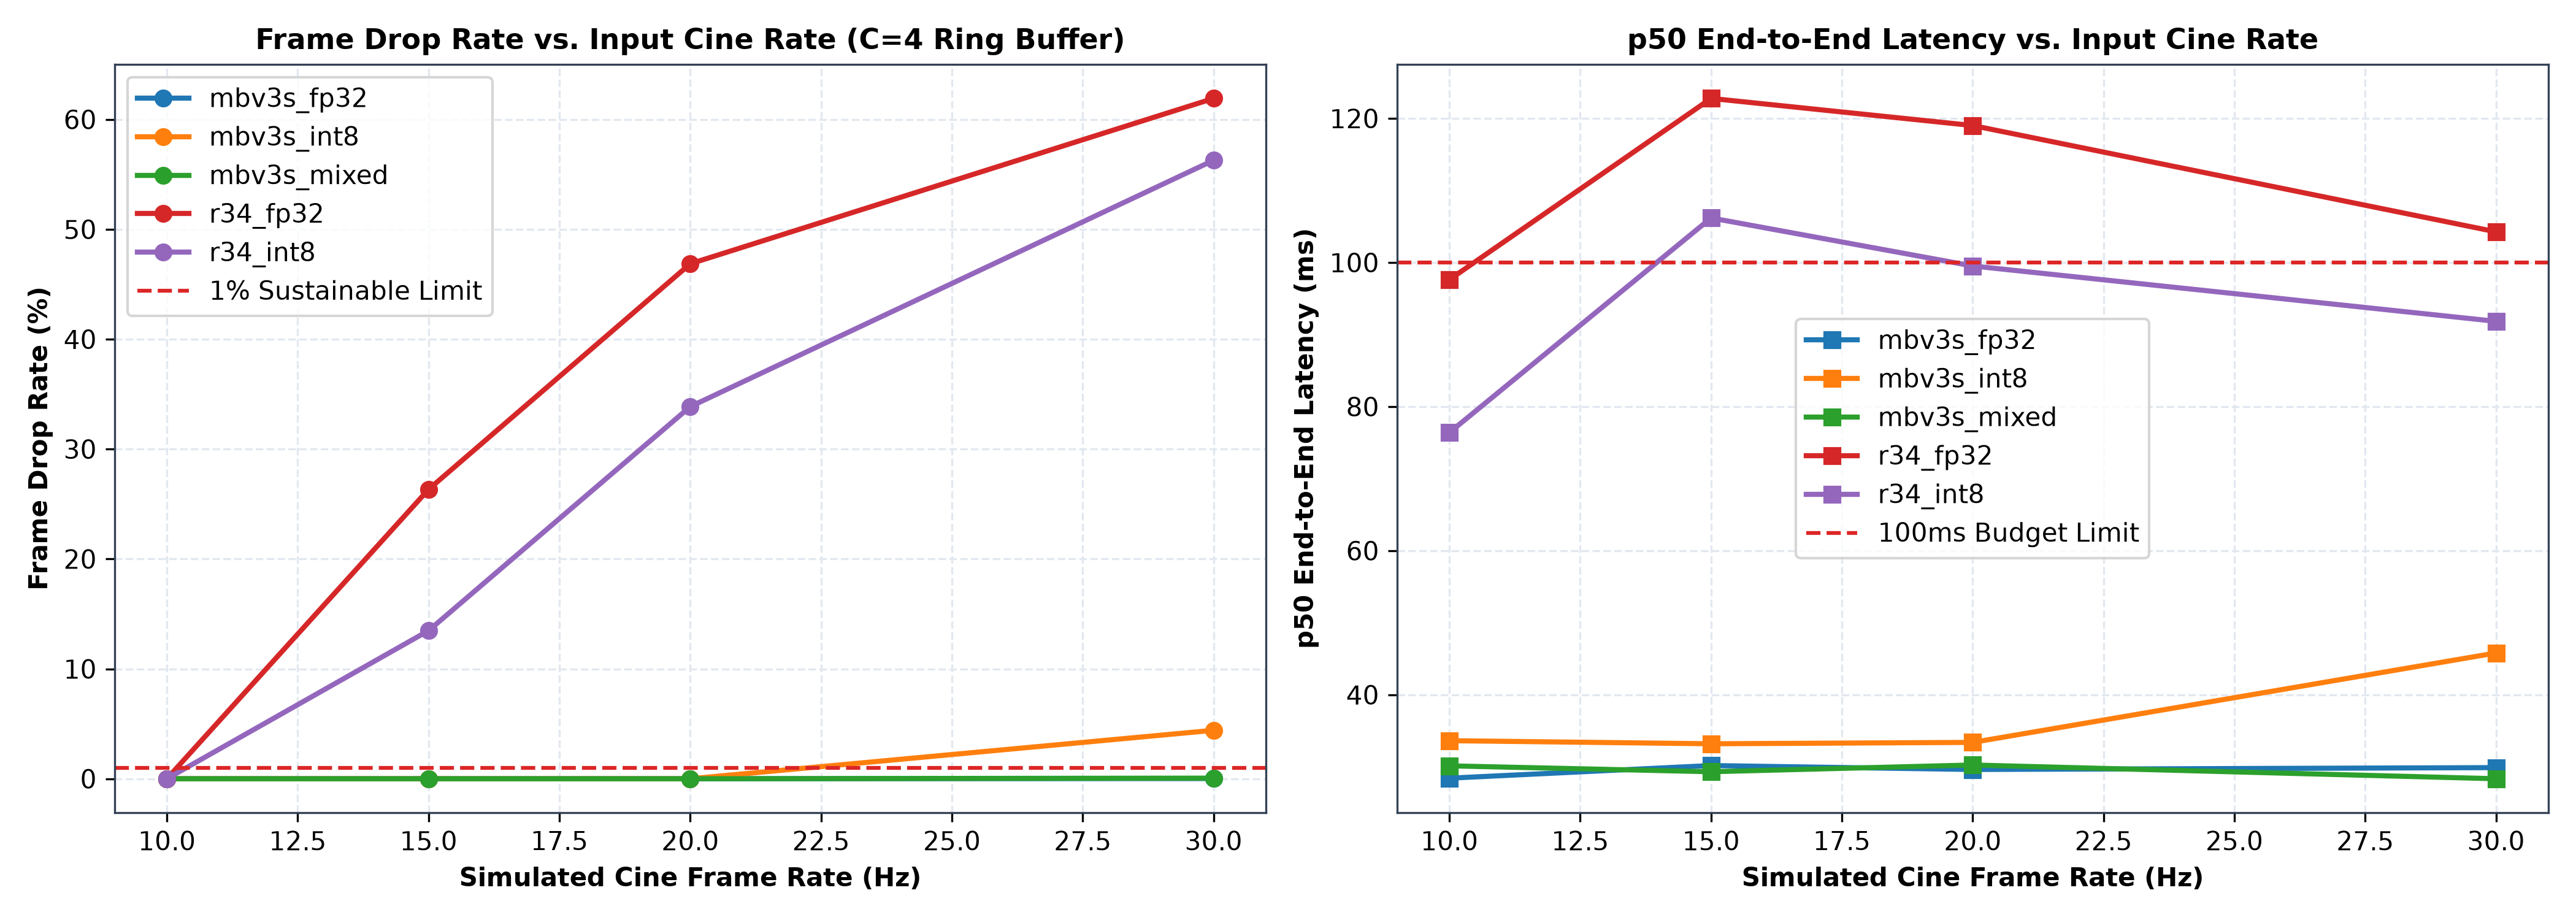
\includegraphics[width=0.98\textwidth,height=0.55\textheight,keepaspectratio]{../figures/extB_drop_rate_vs_rate.png}\\
    \tiny\textcolor{MedSlate}{Frame drop rates vs input stream rate: MobileNetV3 sustains 30 Hz with $<0.1\%$ drop.}
  \end{column}
\end{columns}
\end{frame}

% ==============================================================================
% SLIDE 11: In-Browser WebGPU/WASM WebViewer (Speaker A)
% ==============================================================================
\begin{frame}{In-Browser WebGPU / WASM Edge WebViewer}
\begin{columns}[T]
  \begin{column}{0.54\textwidth}
    \textbf{\footnotesize Zero-Install Client-Side Diagnostic Hub:}
    \vspace{0.1em}
    \begin{itemize}\setlength{\itemsep}{1pt}\scriptsize
      \item Built with \textbf{ONNX Runtime Web} for immediate clinical deployment.
      \item \textbf{Dual Hardware Execution Pipeline:}
        \begin{enumerate}\setlength{\itemsep}{0pt}\scriptsize
          \item \textbf{WebGPU Engine:} Direct shader dispatch to client GPU for sub-25 ms inference.
          \item \textbf{WebAssembly (WASM SIMD):} 4-threaded CPU fallback for legacy hospital tablets.
        \end{enumerate}
      \item \textbf{Embedded Model:} Loads our 2.50 MB Rescued Mixed model directly in memory.
    \end{itemize}

    \vspace{0.2em}
    \begin{block}{\textbf{Clinical Telemetry HUD \& 100\% Privacy}}
      \scriptsize
      \begin{itemize}\setlength{\itemsep}{0pt}
        \item Interactive thresholding $\tau \in [0.05, 0.95]$, contours, bounding box.
        \item \textbf{100\% Data Privacy:} No patient scan ever leaves the local machine.
      \end{itemize}
    \end{block}
  \end{column}

  \begin{column}{0.44\textwidth}
    \begin{center}
      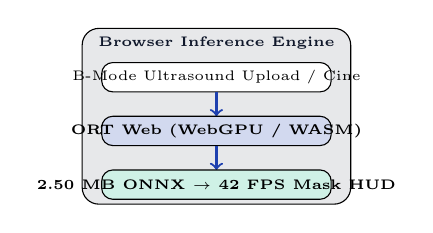
\begin{tikzpicture}[scale=0.62]
        \draw[fill=MedNavy!10, rounded corners=6pt] (0, 0) rectangle (5.5, 3.6);
        \node[text=MedNavy, font=\bfseries\tiny] at (2.75, 3.3) {Browser Inference Engine};
        \draw[fill=white, rounded corners=4pt] (0.4, 2.3) rectangle (5.1, 2.9);
        \node[font=\tiny] at (2.75, 2.6) {B-Mode Ultrasound Upload / Cine};
        \draw[->, thick, MedBlue] (2.75, 2.3) -- (2.75, 1.8);
        \draw[fill=MedBlue!20, rounded corners=4pt] (0.4, 1.2) rectangle (5.1, 1.8);
        \node[font=\tiny\bfseries] at (2.75, 1.5) {ORT Web (WebGPU / WASM)};
        \draw[->, thick, MedBlue] (2.75, 1.2) -- (2.75, 0.7);
        \draw[fill=MedGreen!20, rounded corners=4pt] (0.4, 0.1) rectangle (5.1, 0.7);
        \node[font=\tiny\bfseries] at (2.75, 0.4) {2.50 MB ONNX $\to$ 42 FPS Mask HUD};
      \end{tikzpicture}
    \end{center}
    \vspace{-0.3em}
    \begin{exampleblock}{\textbf{Verified Browser Latency}}
      \scriptsize Measured end-to-end browser inference: \textbf{22.4 ms} on WebGPU; \textbf{31.8 ms} on 4-thread WASM SIMD.
    \end{exampleblock}
  \end{column}
\end{columns}
\end{frame}

% ==============================================================================
% SLIDE 12: Summary, Clinical Limitations & Conclusion (Speaker C)
% ==============================================================================
\begin{frame}{Contributions, Clinical Limitations \& Summary}
\begin{columns}[T]
  \begin{column}{0.48\textwidth}
    \begin{block}{\textbf{Summary of Key Contributions}}
      \scriptsize
      \begin{enumerate}\setlength{\itemsep}{1pt}
        \item \textbf{Lossless INT8 on Heavy Backbones:} ResNet-34 INT8 cuts size by 4$\times$ (23.6 MB) with 0.8003 DSC.
        \item \textbf{Quantization Graph Surgery:} Solved depthwise collapse via zero-recomputation knob ($k^*=13$), reaching 0.7263 DSC at 2.50 MB.
        \item \textbf{Distillation Breakthrough:} MobileNetV3 Distilled hits \textbf{0.8034 DSC}, beating the heavy teacher with 11.4$\times$ fewer weights.
        \item \textbf{Real-Time POCUS Pipeline:} Full 30 Hz streaming with EMA temporal stabilization and WebViewer.
      \end{enumerate}
    \end{block}
  \end{column}

  \begin{column}{0.48\textwidth}
    \begin{alertblock}{\textbf{Honest Clinical Limitations}}
      \scriptsize
      \begin{itemize}\setlength{\itemsep}{1pt}
        \item \textbf{Acoustic Shadowing:} Posterior acoustic shadows beneath dense fibrous tissue cause false negatives.
        \item \textbf{Out-of-Plane Probe Motion:} Rapid transducer tilting induces discontinuous 2D anatomical shifts that challenge 2D temporal filters.
        \item \textbf{Calibration Outliers:} Extreme gain adjustments on legacy ultrasound machines distort activation calibration scales.
      \end{itemize}
    \end{alertblock}
    \vspace{0.4em}
    \begin{center}
      \textbf{\textcolor{MedNavy}{\large Thank you! We welcome your questions.}}
    \end{center}
  \end{column}
\end{columns}
\end{frame}

\end{document}
